
\section{Tafel ronde 2: Wie is het?}
Freddy heeft een paar mooie foto's gevonden van het home Astrid presidium. Kan jij raden wie het is?

Enkel voornaam, fonentisch geschreven
\begin{questions}
\question[1] {
\begin{center}
{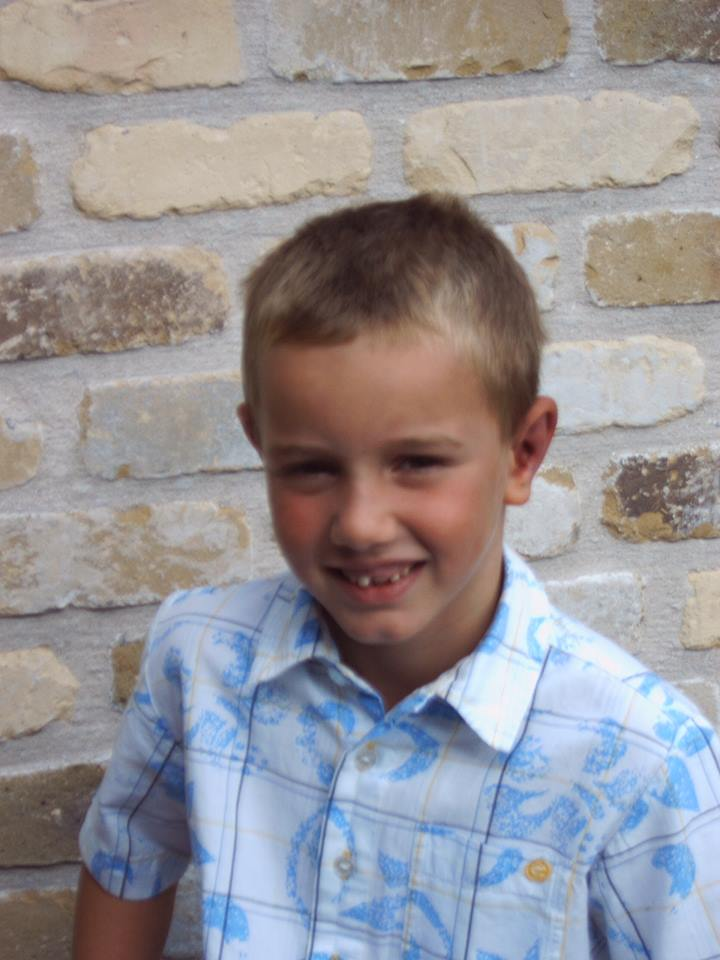
\includegraphics[scale=0.20]{robbe}}
\end{center}
\begin{flushleft}
\makebox[\textwidth]{naam:Robbe}
\end{flushleft} }
\question[1] {
\begin{center}
{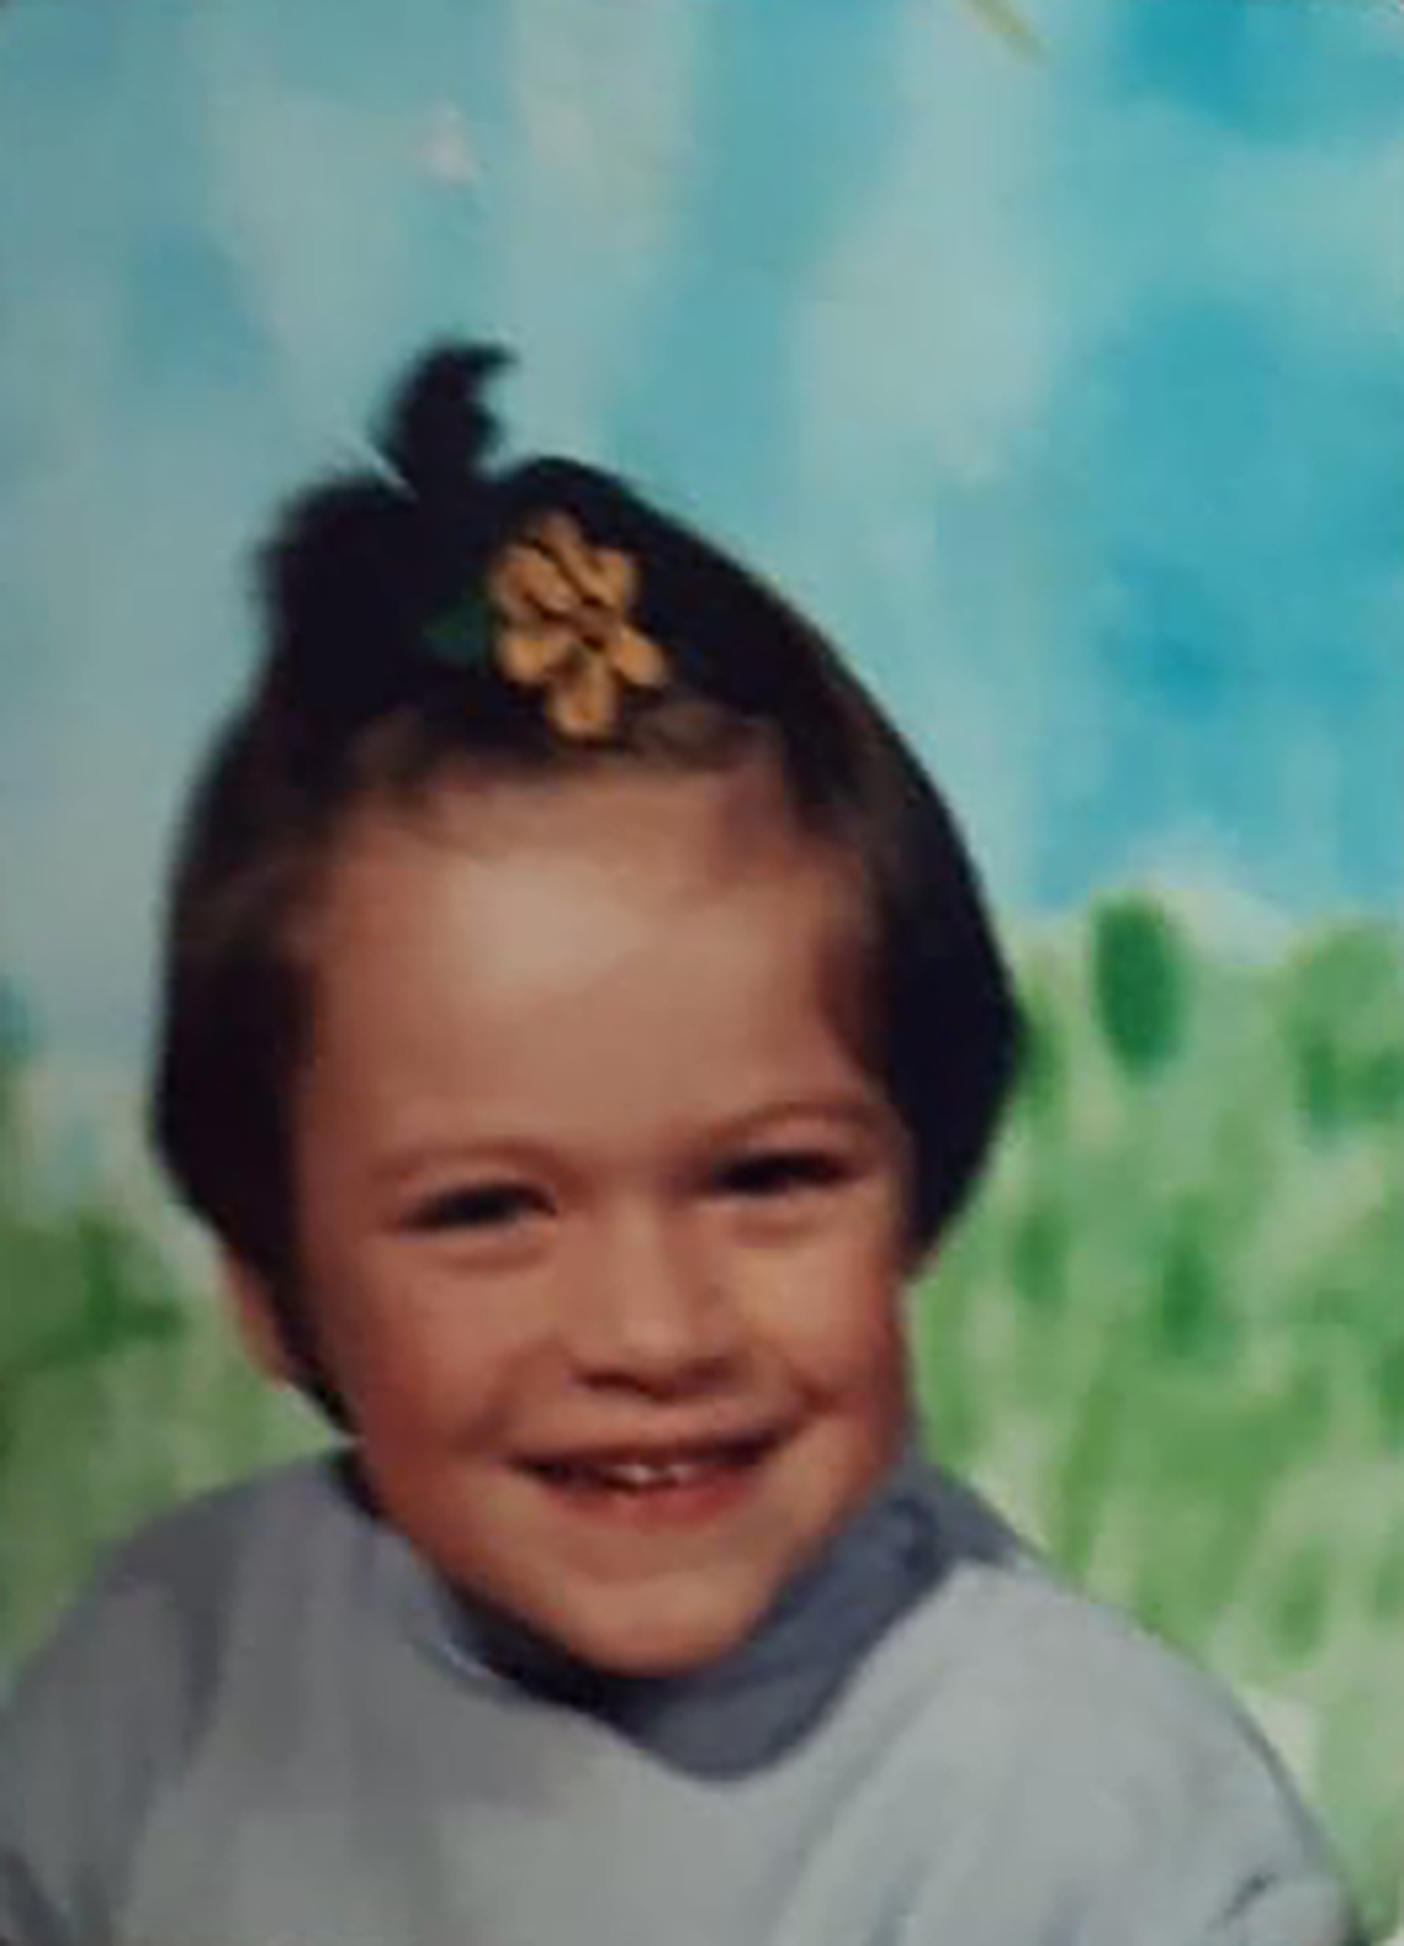
\includegraphics[scale=0.08]{lisa}}
\end{center}
\begin{flushleft}
\makebox[\textwidth]{naam:Lisa}
\end{flushleft} }
\question[1] {
\begin{center}
{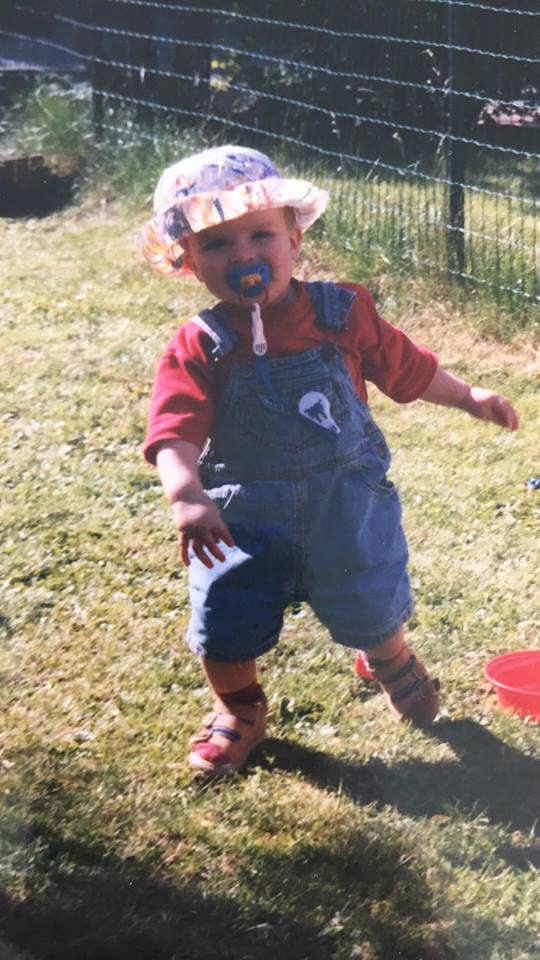
\includegraphics[scale=0.20]{arend}}
\end{center}
\begin{flushleft}
\makebox[\textwidth]{naam:Arend}
\end{flushleft} }
\question[1] {
\begin{center}
{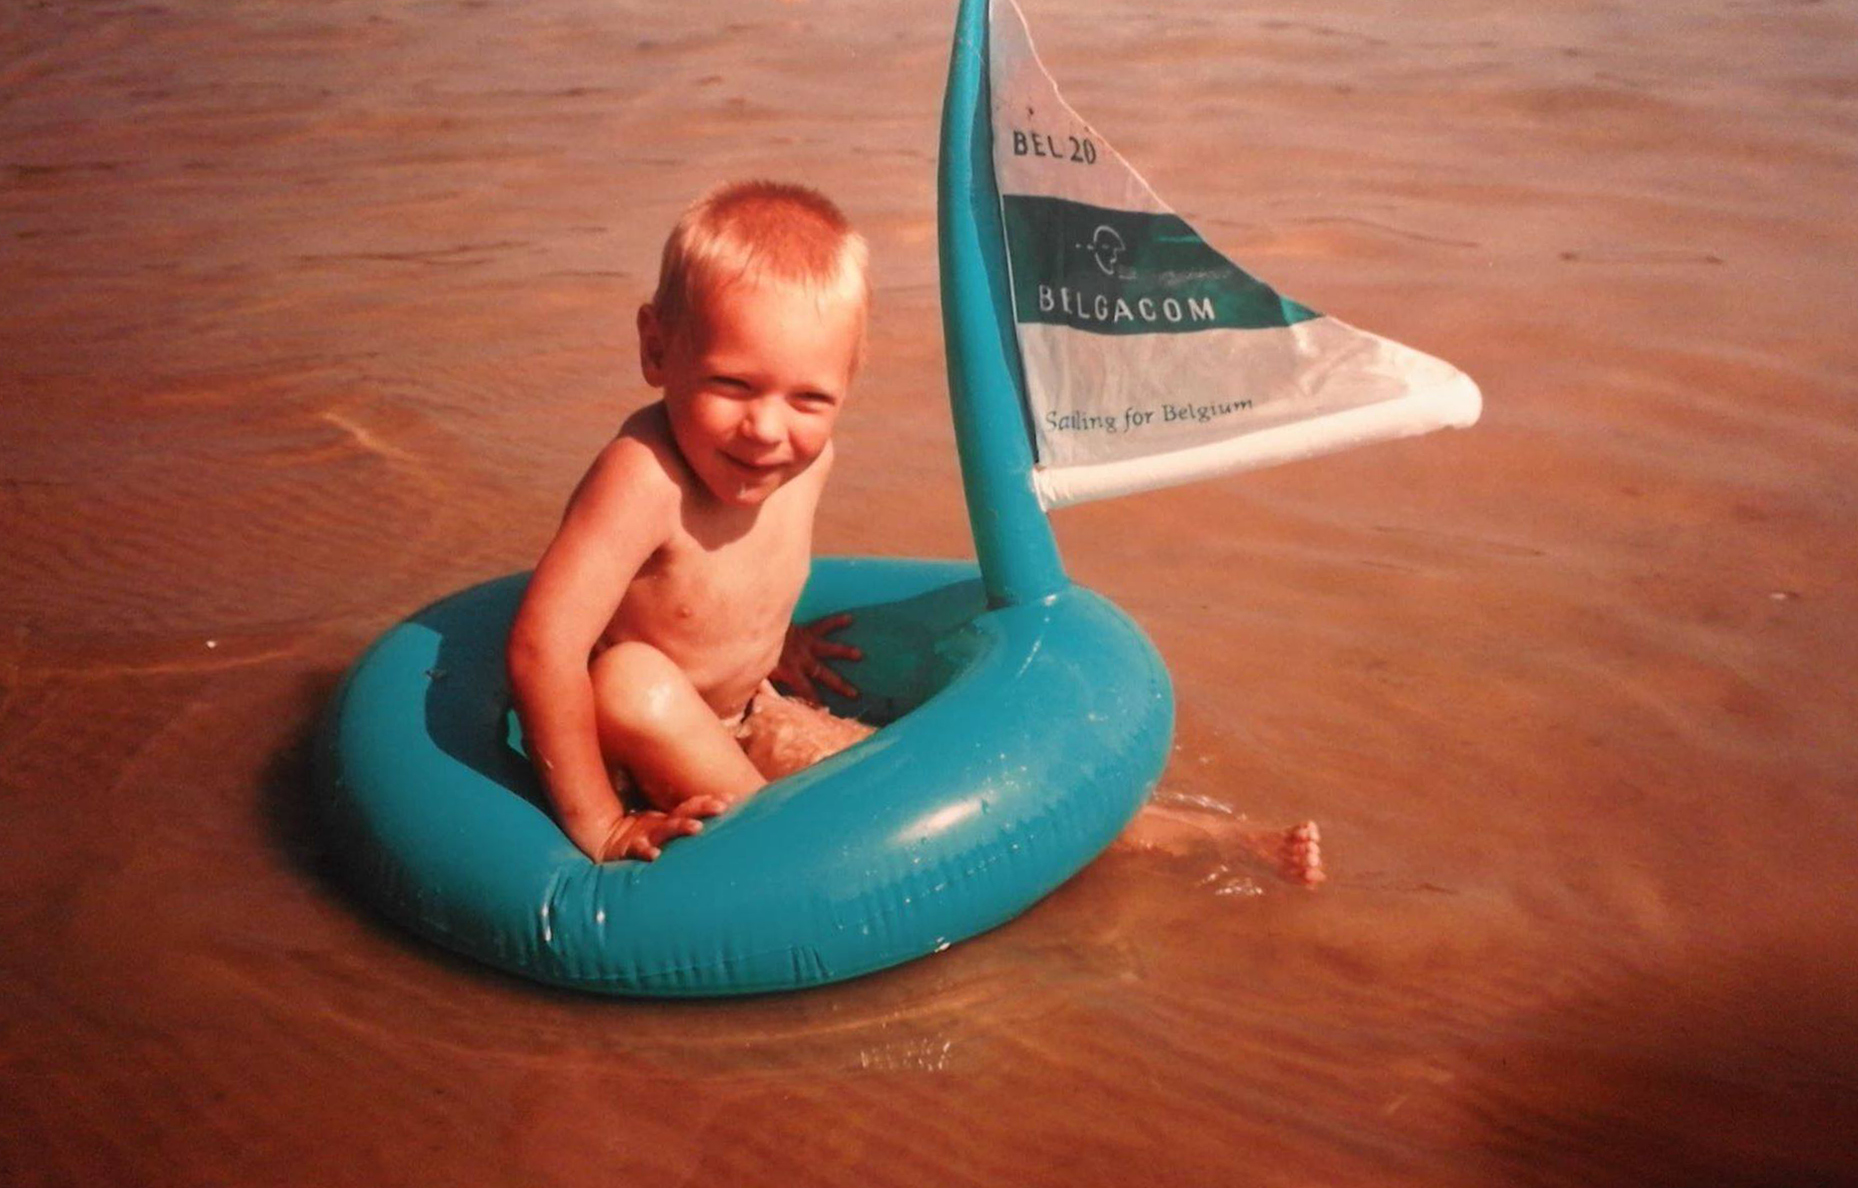
\includegraphics[scale=0.10]{bart}}
\end{center}
\begin{flushleft}
\makebox[\textwidth]{naam:Bart}
\end{flushleft} }
\question[1] {
\begin{center}
{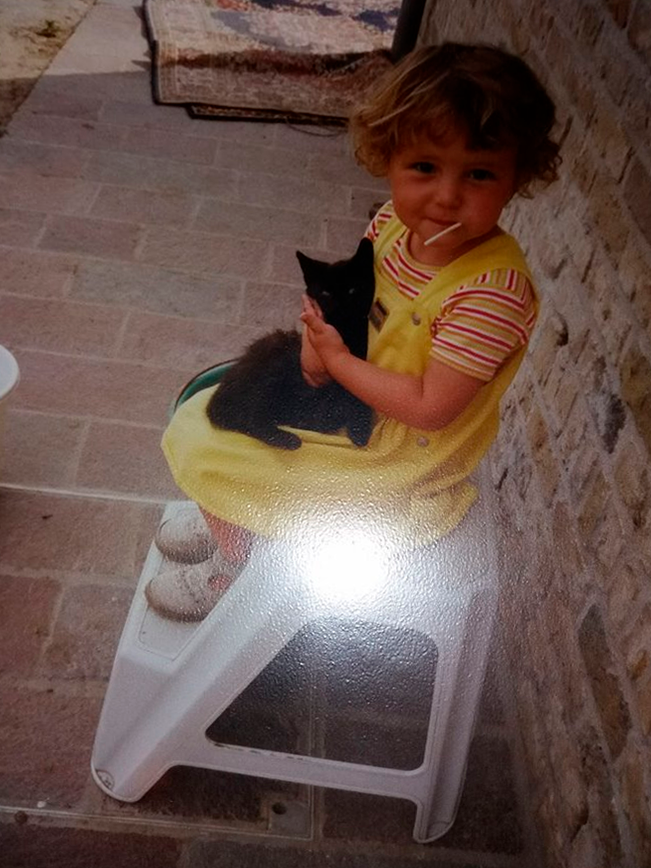
\includegraphics[scale=0.20]{michelle}}
\end{center}
\begin{flushleft}
\makebox[\textwidth]{naam:Michelle}
\end{flushleft} }
\question[1] {
\begin{center}
{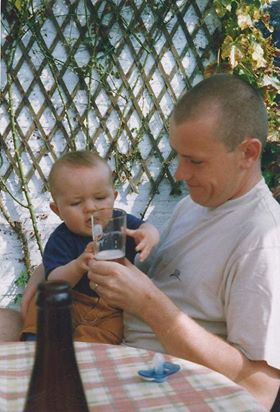
\includegraphics[scale=0.40]{lemmy}}
\end{center}
\begin{flushleft}
\makebox[\textwidth]{naam:Lemmy}
\end{flushleft} }
\question[1] {
\begin{center}
{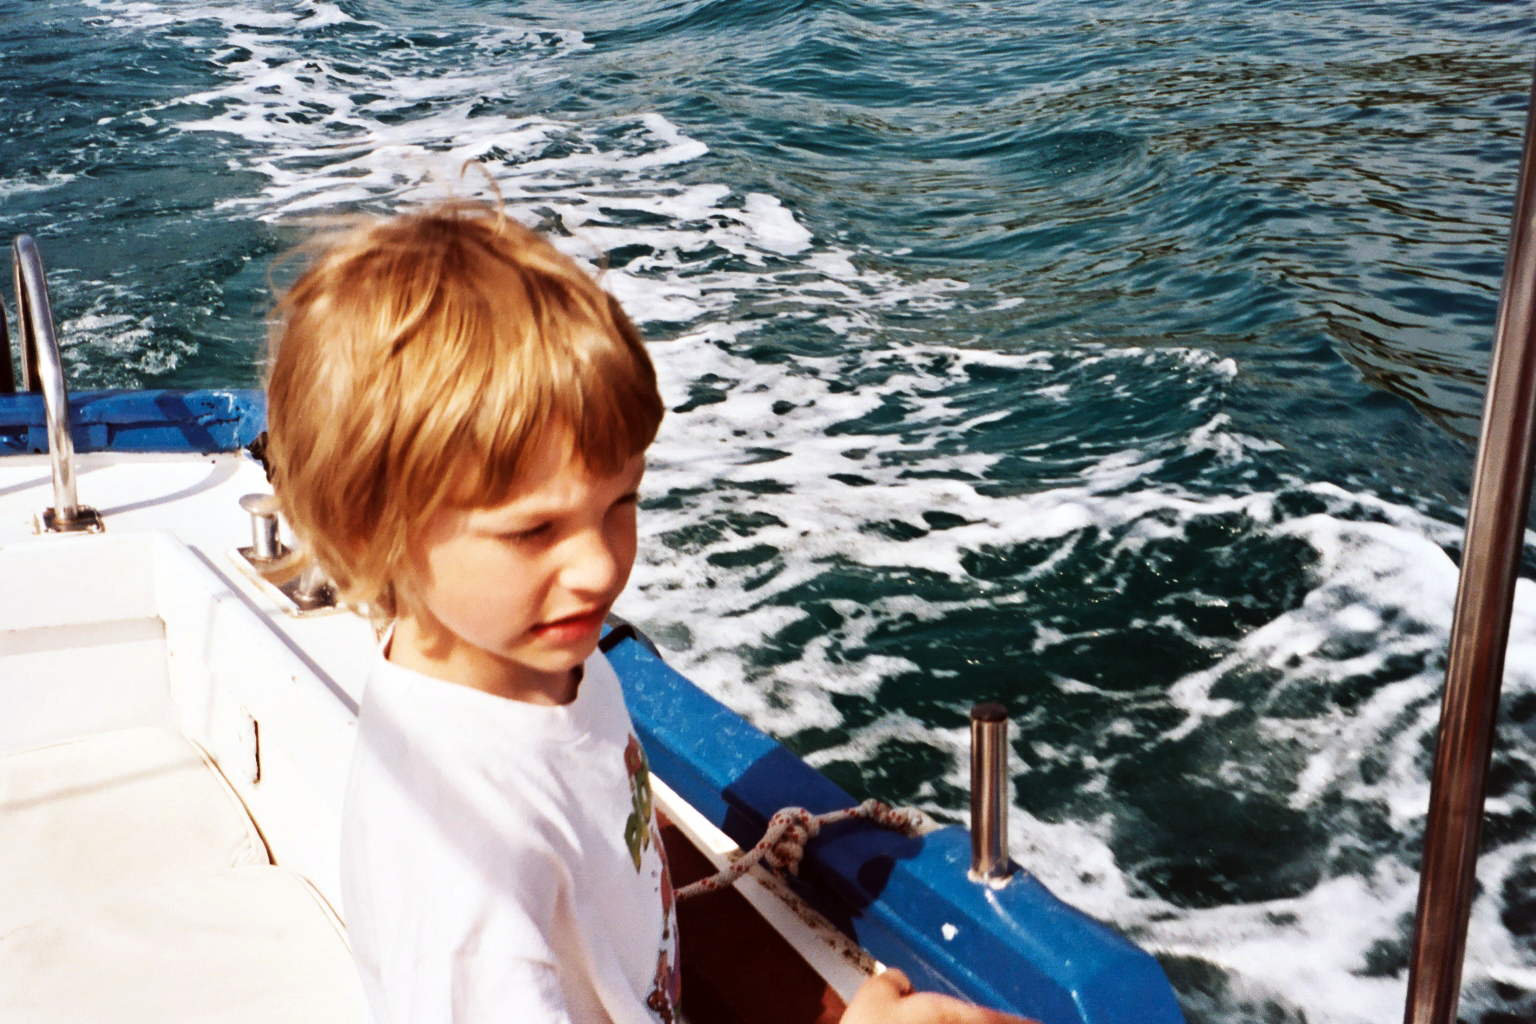
\includegraphics[scale=0.40]{tibo}}
\end{center}
\begin{flushleft}
\makebox[\textwidth]{naam:Tibo of Tibi of Tibidibi}
\end{flushleft} }
\question[1] {
\begin{center}
{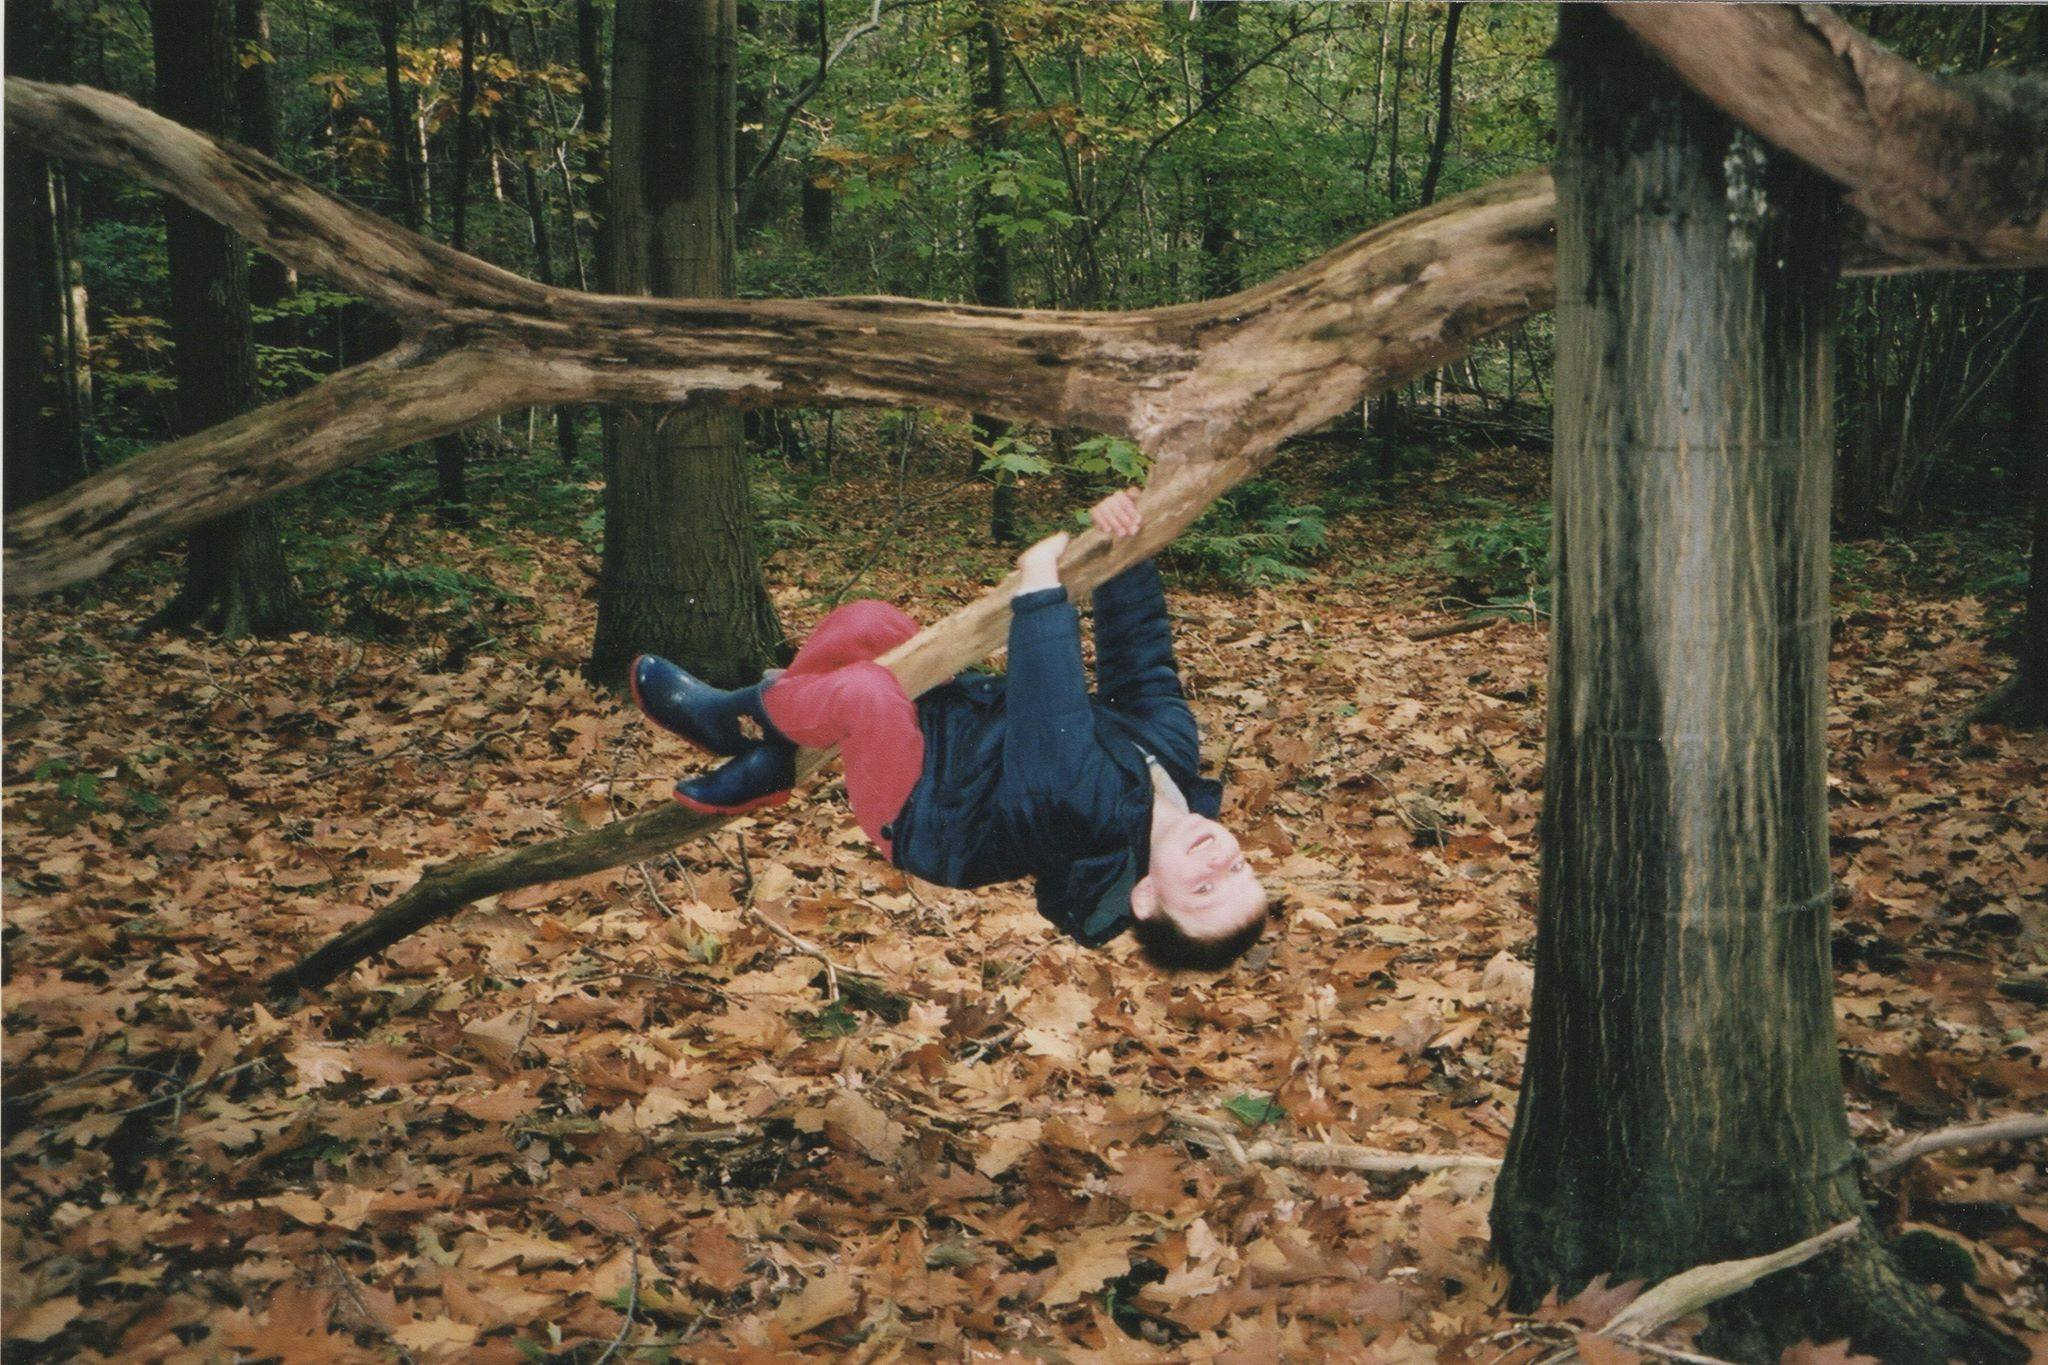
\includegraphics[scale=0.10]{wouter}}
\end{center}
\begin{flushleft}
\makebox[\textwidth]{naam:Wouter}
\end{flushleft} }
\question[1] {
\begin{center}
{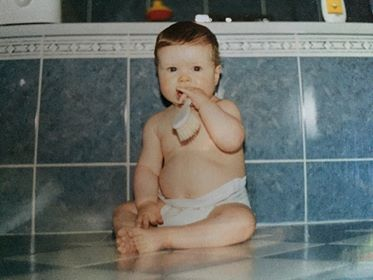
\includegraphics[scale=0.40]{elien}}
\end{center}
\begin{flushleft}
\makebox[\textwidth]{naam:Elien}
\end{flushleft} }
\question[1] {
\begin{center}
{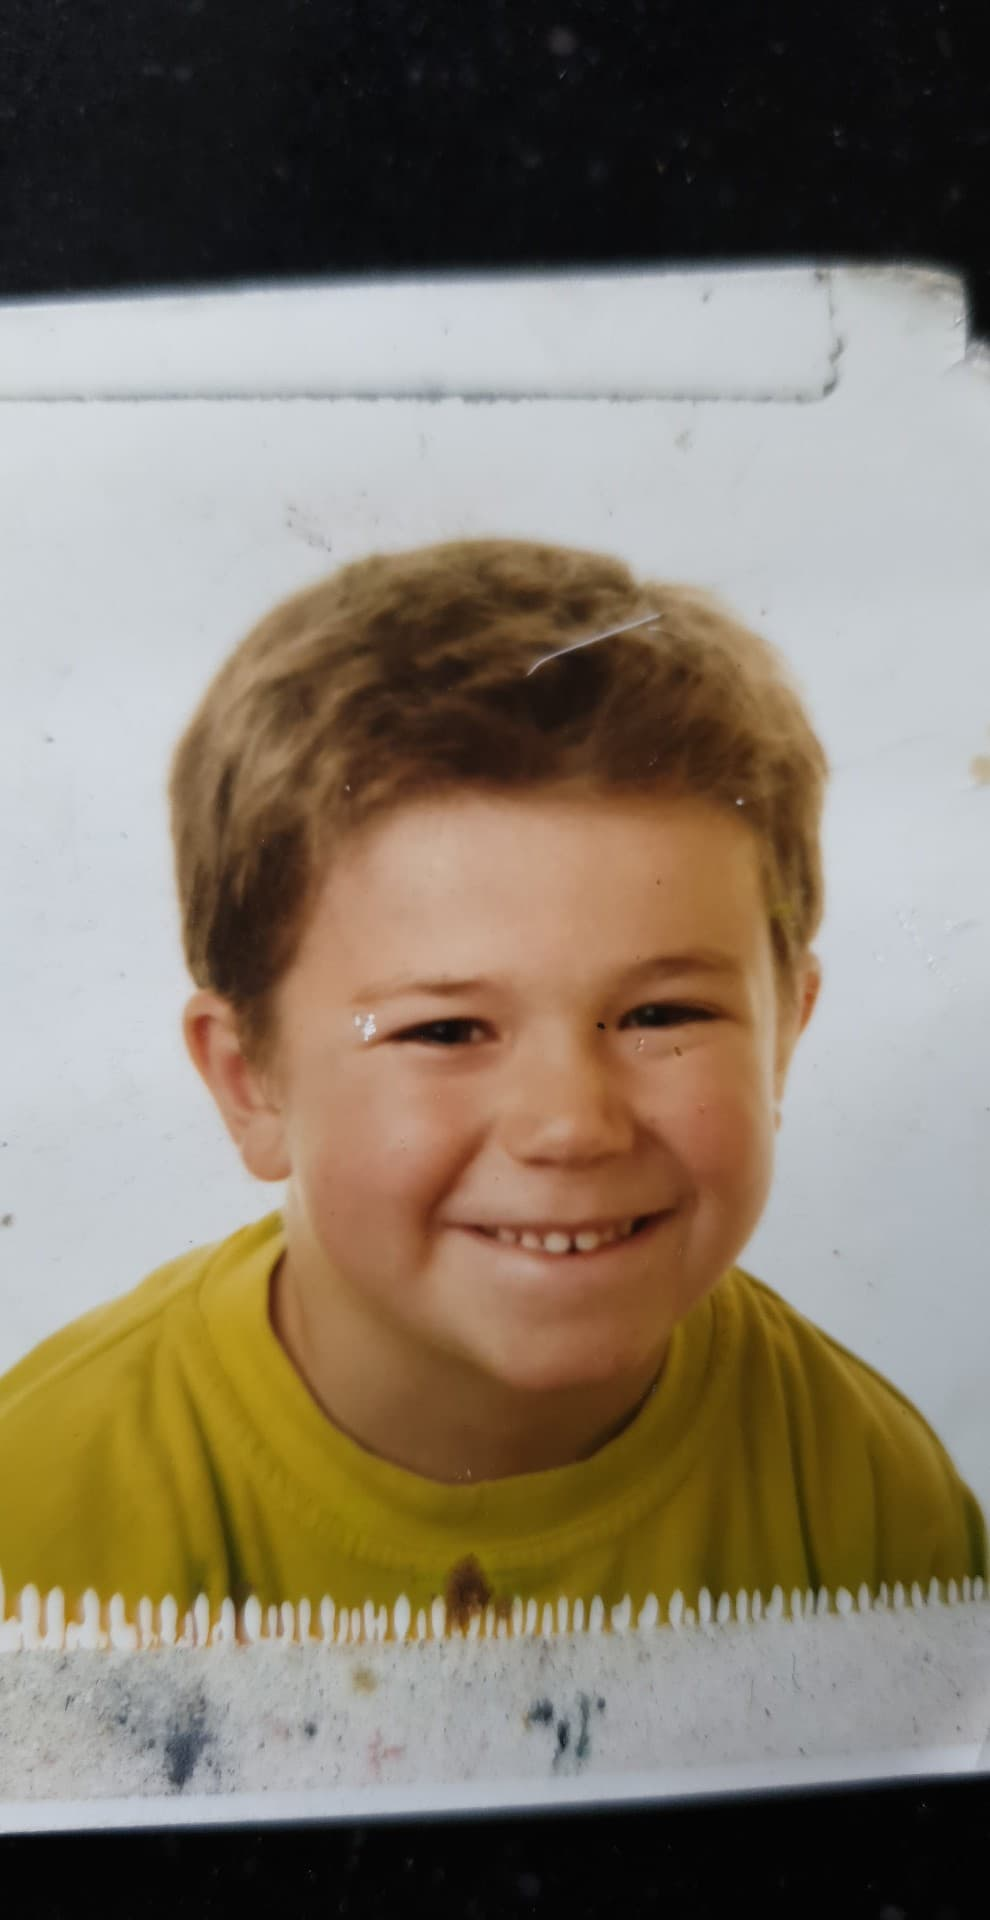
\includegraphics[scale=0.10]{sander}}
\end{center}
\begin{flushleft}
\makebox[\textwidth]{naam:Sander}
\end{flushleft} }

\end{questions}
\newpage